\documentclass[a4paper]{article}
%\usepackage{vntex}
%\usepackage[english,vietnam]{babel}
\usepackage[utf8]{vietnam}

\usepackage{multirow} %enable mutirow
\usepackage{array} % enable us to define new content format in table
\newcolumntype{P}[1]{>{\centering\arraybackslash}p{#1}}
\newcolumntype{M}[1]{>{\centering\arraybackslash}m{#1}}

\usepackage[linesnumbered,lined,ruled,commentsnumbered]{algorithm2e}

\makeatletter
\def\BState{\State\hskip-\ALG@thistlm}
\makeatother
\usepackage{tabularx}
\usepackage{a4wide,amssymb,epsfig,latexsym,multicol,array,hhline,fancyhdr}
\usepackage{float}
\restylefloat{table}
\usepackage{amsmath}
\usepackage{lastpage}
%\usepackage[lined,boxed,commentsnumbered]{algorithm2e}

%use new enum package
\usepackage{enumitem}
\usepackage{color}
\usepackage{graphicx}							% Standard graphics package
\usepackage{array}
\usepackage{tabularx, caption}
\usepackage{multirow}
\usepackage{multicol}
\usepackage{rotating}
\usepackage{graphics}
\usepackage{geometry}
\usepackage{setspace}
\usepackage{epsfig}
\usepackage{booktabs}% http://ctan.org/pkg/booktabs
\newcommand{\tabitem}{~~\llap{\textbullet}~~}
\usepackage{tikz}
\usetikzlibrary{arrows,snakes,backgrounds}
\usepackage{hyperref}
\hypersetup{urlcolor=blue,linkcolor=black,citecolor=black,colorlinks=true} 
%\usepackage{pstcol} 								% PSTricks with the standard color package

\newcommand{\matr}[1]{\mathbf{#1}}
\renewcommand{\vec}[1]{\mathbf{#1}}
\newcommand{\code}[1]{\texttt{#1}}
\DeclareMathOperator*{\argmax}{\arg\!\max}
\renewcommand*\descriptionlabel[1]{\hspace\leftmargin$#1$}
%\DeclarePairedDelimiter\abs{\lvert}{\rvert}
\usepackage{siunitx}
\relpenalty=10000
\binoppenalty=10000
\usepackage{listings}

\usepackage{fancyhdr}
\setlength{\headheight}{40pt}
\pagestyle{fancy}
\fancyhead{} % clear all header fields
\fancyhead[L]{
 \begin{tabular}{rl}
    \begin{picture}(25,15)(0,0)
    \put(0,-8){
\includegraphics[width=8mm, height=8mm]{hcmut.png}}
    %\put(0,-8){\epsfig{width=10mm,figure=hcmut.eps}}
   \end{picture}&
	%
\includegraphics[width=8mm, height=8mm]{hcmut.png} & %
	\begin{tabular}{l}
		\textbf{\bf \ttfamily Ho Chi Minh University of Technology}\\
		\textbf{\bf \ttfamily Department of Computer Science and Engineering}
	\end{tabular} 	
 \end{tabular}
}
\fancyhead[R]{
	\begin{tabular}{l}
		\tiny \bf \\
		\tiny \bf 
	\end{tabular}  }
\fancyfoot{} % clear all footer fields
\fancyfoot[L]{\scriptsize \ttfamily Assignment for Computer Architecture - Year 2019 - 2020}
\fancyfoot[R]{\scriptsize \ttfamily Page {\thepage}/\pageref{LastPage}}
\renewcommand{\headrulewidth}{0.3pt}
\renewcommand{\footrulewidth}{0.3pt}


%%%
\setcounter{secnumdepth}{4}
\setcounter{tocdepth}{3}
\makeatletter
\newcounter {subsubsubsection}[subsubsection]
\renewcommand\thesubsubsubsection{\thesubsubsection .\@alph\c@subsubsubsection}
\newcommand\subsubsubsection{\@startsection{subsubsubsection}{4}{\z@}%
                                     {-3.25ex\@plus -1ex \@minus -.2ex}%
                                     {1.5ex \@plus .2ex}%
                                     {\normalfont\normalsize\bfseries}}
\newcommand*\l@subsubsubsection{\@dottedtocline{3}{10.0em}{4.1em}}
\newcommand*{\subsubsubsectionmark}[1]{}
\makeatother

%long table
\usepackage{ltablex}

\usepackage{listings}
\lstset{basicstyle=\ttfamily,
  showstringspaces=false,
  commentstyle=\color{red},
  keywordstyle=\color{blue},
  frame=single,
}

\begin{document}
\begin{titlepage}
   
\begin{center}
VIET NAM NATIONAL UNIVERSITY, HO CHI MINH CITY \\
HO CHI MINH UNIVERSITY OF TECHNOLOGY\\
DEPARTMENT OF COMPUTER SCIENCE AND ENGINEERING 
\end{center}

\vspace{1cm}

\begin{figure}[h!]
\begin{center}

\includegraphics[width=3cm]{hcmut.png}
\end{center}
\end{figure}

\vspace{1cm}


\begin{center}
\begin{tabular}{c}
\multicolumn{1}{l}{\textbf{{\Large OPERATING SYSTEM}}}\\
~~\\
\hline
\\
\multicolumn{1}{l}{\textbf{{\Large Assignment 1}}}\\
\\
\textbf{{\Huge System Call}}\\
\\
\hline
\end{tabular}
\end{center}

\vspace{3cm}

\begin{table}[h]
\begin{tabular}{rrl}
\hspace{5 cm} & Instructor: & Nguyễn Minh Trí\\
& Student: & Trần Hoàng Long - 1852545 \\
\end{tabular}
\end{table}

\begin{center}
{\footnotesize Ho Chi Minh City, May 2020}
\end{center}
\end{titlepage}


%\thispagestyle{empty}

\newpage
\tableofcontents
\newpage
\section{Introduction}
This paper is the report for the work of compiling a linux kernel and implementing a system call inside that kernel.\\
The base kernel used to build our custom one is linux-4.4.56\\
The operating system is Ubuntu 12.04 32-bit\\
The initial kernel of the OS is linux 3.11.0-26-generic\\
The process of implementing a system call (details later) and compiling, installing our custom kernel, overriding the original one from the OS is described step by step in sections of this assignment.
\section{Adding new system call}
\subsection{Operating system and kernel preparation}
First step, of course is to get the Operation needed. I went with Ubuntu 12.04 32-bit and installed it as a virtual machine using the Virtual Box emulator.\\
Next is to install the needed packages for our work:
\begin{lstlisting}[language=bash]
#updating kernel and the current installed packages
$ sudo apt-get update

#essential package coding and compiling files (gcc, make,..)
$ sudo ap-get install build-essential

#essential package for building kernel
$ sudo apt-get install kernel-package
\end{lstlisting}
\textbf{QUESTION:} Why do we need to install kernel-package?\\\\
\textbf{Answer:} Kernel package is a system to create kernel related packages and it's an upgrade, a more automated tool for the job of compiling and installing a custom kernel, instead of the older manual method, which includes many steps in order.\\
Now thanks to the kernel-package, all those many steps are all handled by this package. That's the main reason we use this package for our assignment. \\
It also provide many other features like kernel management and different support tools but that, i think is outside the scope of the assignment.\\\\
Last prep step is getting the base kernel that we will modify and compile then install, overriding the current kernel (3.11.0-26-generic).\\
Our base kernel is linux-4.4.56, download it into a folder and extract the file (extract with option -xvJf). Link: \url{https://mirrors.edge.kernel.org/pub/linux/kernel/v4.x/linux-4.4.56.tar.xz}\\\\
\textbf{\textit{Note:}} From now, the directory that we just got from un-packing the file (...../linux-4.4.56/) will be referred to as the \textbf{kernel directory}.\\\\
\textbf{QUESTION:} Why do we have to use another kernel source and not compile the original kernel directly?\\\\
\textbf{Answer:} The original kernel on our operating system is in the binary form, already pre-compiled for us to install in our OS. So, we can still make change to it (though very difficult) but we can not compile it, since, clearly it's already is compiled and installed.\\
So in order to make change to the system's kernel we need to download an external kernel source code, make change to that and compile it in. Then install to our system to reflect the changes.\\

\subsection{Kernel configuration}
Step 1: Take the system's current kernel's configuration and copy that to our custom kernel.
\begin{lstlisting}[language=bash]
$ cp /boot/config/config-<current_kernel_version> <kernel_dir>
#you can find the current kernel version by "uname -r"
\end{lstlisting}
Step 2: Change the custom kernel's name to something else to avoid problems. We'll change it into "<current\_name>.MSSV"
\begin{lstlisting}[language=bash]
#install package needed for chaging the kernel configuration
$ sudo apt-get install libncurses5-dev

#go to the kernel's directory and call this
$ make nconfig #or make menuconfig
\end{lstlisting}
In the pop-up configuration option menu, go to General setup and then choose the line Local version - append to kernel release. Then, type in a dot ".", followed by your MSSV.
\begin{center}
    \begin{figure}[H]
    \begin{center}
     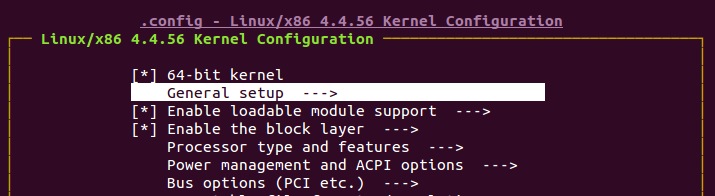
\includegraphics[scale=1]{make_nconfig.png}
    \end{center}
    \caption{Choose general setup}
    \end{figure}
\end{center}
\begin{center}
    \begin{figure}[H]
    \begin{center}
     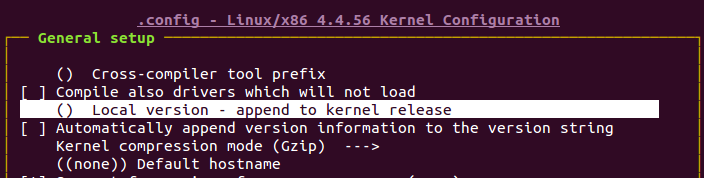
\includegraphics[scale=1]{general_setting.png}
    \end{center}
    \caption{Choose local version - append to kernel release}
    \end{figure}
\end{center}
\begin{center}
    \begin{figure}[H]
    \begin{center}
     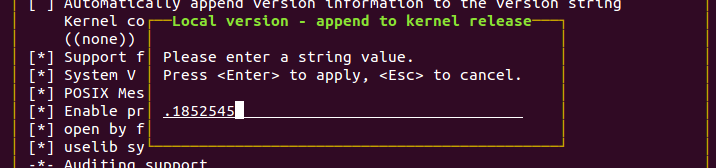
\includegraphics[scale=1]{appendKernelName.png}
    \end{center}
    \caption{My case for the kernel name append}
    \end{figure}
\end{center}
F6 to save and F9 to exit when your're done.
\section{System call Implementation}
\subsection{Pre-testing with module}
Instead of writing the actual kernel code and compile the kernel directly, risking error and a lot of time. You can test it as a system's module (put in different folder from our kernel's directory).\\
I won't go in details here, but a guide can be found \href{http://www.tldp.org/LDP/lkmpg/2.6/html/x40.html}{Here}
\subsection{Prototype}
The prototype of our system call is as follows:
\begin{lstlisting}[language=c]
long procsched(int pid, struct pro_segs* info);
\end{lstlisting}
The user provide a PID for the process to search for and the "info" for outputting the process's schedule data. The system call search for the given process ID and output data into the parameter "info" and return 0 if success, -1 if process not found.
\subsection{Implementation}
\textbf{Step 1:} Adding a new system call entry to our kernel's system call table so that the system knows about the new system call.\\
In our kernel directory, in arch/x86/entry/syscalls, add new system call entry to both files syscall\_32.tbl and syscall\_64.tbl:
\begin{lstlisting}[title=syscall\_32.tbl]
[number]	i386	procsched	sys_procsched
\end{lstlisting}
\begin{lstlisting}[language=c,title=syscall\_64.tbl]
[number]	x32	procsched	sys_procsched
\end{lstlisting}
\textbf{Note:} $[number]$ is the next entry id in the table. In my case, the id was 377 for syscall\_32.tbl and 546 for syscall\_64.tbl\\\\
\textbf{QUESTION:} What is the meaning of other parts in the file 
syscall\_32.tbl and syscall\_64.tbl, i.e: i386, procsched and sysprocsched?\\\\
\textbf{Answer:} In those two files, the format of a system call entry is defined as follows:
\begin{center}
$<number> <abi> <name> <entry\_point>$ (all separated by TAB symbols).
\end{center}
\begin{enumerate}
\item $<number>$: is like the id of the system call, we can provoke the call if we know the entry number.
\item $<abi>$: This attribute specifies the type of entry of our system call for the kernel's ABI (ABI and this field will be explained more detailed later).
\item $<name>$: This is the name of our system call
\item $<entry\_point>$: This is the name of the function, the object file that actually implement our system call. For convention, this is named as "sys\_$<system call name>$".
\item $<compat\_entry\_point>$: This is another field that's only in the file syscall\_32.tbl. It is the entry point for i386 ABI emulation on x86-64 kernel. (not the scope of this assignment)
\end{enumerate}
\textbf{More on ABI and $<abi>$ field in the syscalls table:}\\
ABI is short for "Application Binary Interface". It's job is to define data structures and methods that our program's compiled \textbf{\emph{machine code}} uses to access external library. It also define how code is stored in library file so that program using the library can locate the method it's calling and execute that. Just think ABI is the API of machine code, similar, but on a lower level.\\
Now back to the field $<abi>$ in our syscalls table.\\\\
There's 3 different ABIs:
\begin{itemize}
\item i386 ABI is 32-bit ABI for 32-bit x86 kernel
\item x86-64 ABI is 64-bit ABI for 64-bit x86 kernel
\item x32 ABI is 32-bit ABI for 64-bit x86 kernel
\end{itemize} 
And in our syscalls table, we need to specify the type of ABI that's for our syscall entry using the field $<abi>$.
\begin{itemize}
\item For 64-bit processor, specified in file "syscall\_64.tbl", we have option "64" for x86-64 ABI, option "x32" for x32 ABI and option "common" for both of them.
\item For 32-bit processor, specified in file "syscall\_32.tbl", we only have option "i386" for the i386 ABI.
\end{itemize}\ \\
\textbf{Step 2:} Declaring the system call itself\\
We need a declaration of the system call in the file include/linux/syscall.h in our kernel's directory. Append at the end of syscall.h:
\begin{lstlisting}[language=c]
struct proc_segs;

asmlinkage long sys_procsched(int pid, struct proc_segs* info);
\end{lstlisting}
\textbf{QUESTION:} What's the meaning of declaring the above lines in include/linux/syscalls.h?\\\\
\textbf{Answer:} First of all, it's necessary to include the information of our system calls in the file syscalls.h because that's where the declarations for system calls are stored.
\begin{enumerate}
\item As for "struct proc\_segs;". This is the "custom" structure that holds schedule data of our process that we need to work with. The further definition is in the .c file.
\item The latter line define prototype of our system call function. \item The keyword "asmlinkage" is a \#define that tells our cpu that the function's arguments will be stored on the stack instead of the register. This is due to the use of "general purpose" registers in our machine. In Linux, we have 6 of these registers an when a function is called, the first 6 arguments are stored in them instead of stack for fast calling. But, it's a little different for system call. You see, when we make a call to a function call with some of our given arguments, the system switch from user mode to kernel mode, and to save the current state, all of the passed parameter must be saved to the stack (even the ones that are in the general purpose register) and this state is restored later. Because of this, instead of looking at the stack and the register for our system call's argument, the "asmlinkage" is use to tell the compiler to look into stack only.
\end{enumerate}\ \\
\textbf{Step 3:} Function implementation\\\\
\textbf{Note:} This is the system call but not the one that user will be calling, this system call will later be wrapped in wrapper code for user easy access.\\
In the kernel directory, go to arch/x86/kernel and create a source file sys\_procsched.c
\begin{lstlisting}[language=c]
#include<linux/linkage.h>
struct proc_segs{
	unsigned long mssv;
	unsigned long pcount;
	unsigned long long run_delay;
	unsigned long long last_arrival;
	unsigned long long last_queued;
};

asmlinkage long sys_procsched(int pid, struct proc_segs * info) {
	// Find task_struct of process with pid given
	// Copy data from task_struct->sched_info to "info"
	// Also adds in MSSV (mine is 1852545)
}
	
\end{lstlisting}
Last step: Adding the file to the Makefile that compiles our system calls. Also in arch/x86/kernel, add line to the end of Makefile.
\begin{lstlisting}[language=bash]
obj-y += sys_procsched.o
\end{lstlisting}
When done, the kernel is ready to go.
\section{Complication and Installation process}
\subsection{Build the configured kernel}
First, run make in the kernel's directory to compile it. This take very long time depending on your processing power. In my case specifically, i use the tag "-j 6" to run this process in 6 parallel cores that i set up for my machine. Took aprox one hour for me.
\begin{lstlisting}[language=bash]
make -j 6
\end{lstlisting}
Next is to build the kernel modules, this can also run in parallel mode.
\begin{lstlisting}[language=bash]
make -j 6 modules
\end{lstlisting}
\textbf{QUESTION:} What's the meaning of the two stage, namely "make" and "make modules"?\\\\
\textbf{ANSWER:}
\begin{itemize}
\item "make": compiles and links the kernel image. The result is a file called vmlinuz.
\item "make modules": compiles all the modules selected in the configuration and link the new object file to the newly made kernel image from step above.
\end{itemize}
\subsection{Install the new kernel}
From the kernel's directory.//
We install the modules first:
\begin{lstlisting}[language=bash]
sudo make -j 6 modules_install
\end{lstlisting}
Then the kernel itself:
\begin{lstlisting}[language=bash]
sudo make -j 6 install
\end{lstlisting}
Reboot after installation is done:
\begin{lstlisting}[language=bash]
sudo reboot
\end{lstlisting}
When back into the system, check the version of your kernel:
\begin{lstlisting}[language=bash]
uname -r
\end{lstlisting}
If the version is "4.4.56.<MSSV>", it's a kernel success. My case is \textbf{"4.4.56.1852545"}.
\subsection{Testing system call}
Write a small program to test the system call we made, as follows:
\begin{lstlisting}[language=c]
#include <sys/syscall.h>
#include <stdio.h>
#define SIZE 10
int main(){
	long sysvalue;
	unsigned long info[SIZE];
	sysvalue = syscall([number_32],1,info);
	printf("My MSSV: %lu\n", info[0]);
}
\end{lstlisting}
This should print your MSSV (that you implemented in the system call) as the result.
\begin{center}
    \begin{figure}[H]
    \begin{center}
     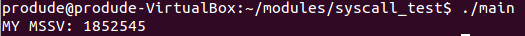
\includegraphics[scale=1]{testProgram.png}
    \end{center}
    \caption{Result of my test program}
    \end{figure}
\end{center}
\textbf{QUESTION:} Why can test program given check whether our system works or not?\\\\
\textbf{ANSWER:} In short, the program above provoked our system call to write data in the array "sysvalue" and when we print it's first element, we get the aligned data, which is our MSSV. This shows that our system call is working properly.\\
For more information, it seems odd that we are passing an array as the argument instead of the actual data struct that we need for the system call.\\
But, in nature, the data aligned in struct is the same as array (the only difference is each element has different container size). So in C, giving array as an argument instead of struct is just like passing a pointer, which is acceptable here. As long as we align the data we need to read properly by declaring the right type for our array, we still can extract data from the struct. Except for ones that are of wrong size and not aligned. Be wary of this data corruption when doing this.\\
In the our system call, the struct is defined with mssv and pcount as type "ulong" and the other 3 as "ulonglong". So when we pass our array with type "ulong", it aligns with mssv and pcount so that can be extracted for use. But for the other 3 fields, data corruption (due to non-alignment) will mess-up the output. Visualization below:
\begin{center}
    \begin{figure}[H]
    \begin{center}
     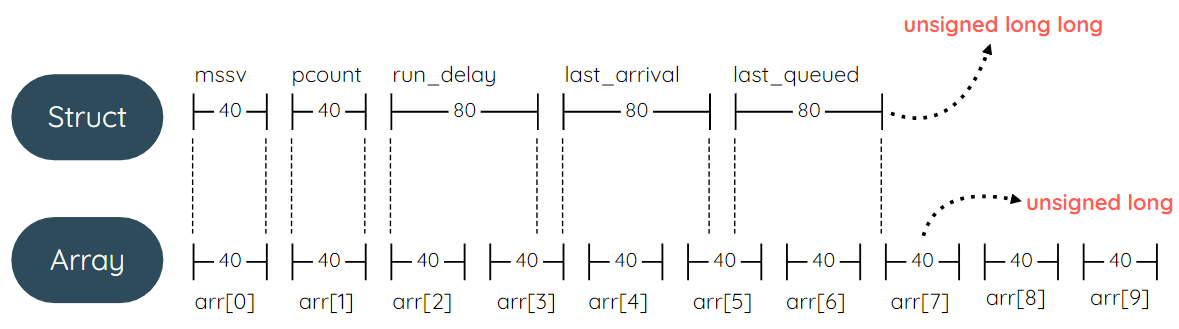
\includegraphics[scale=0.6]{array_struct.png}
    \end{center}
    \caption{Visualization for data alignment when we pass array instead of structure}
    \end{figure}
\end{center}
\section{Making API for system call}
\subsection{Writing wrapper}
As mentioned before, the system call itself if fine, but it's inconvenient for programmer's use, so we will implement wrapper to make it convenient. This is done separated from the kernel, not requiring us to re-compile.\\
First is the header: procsched.h
\begin{lstlisting}[language=c]
#ifndef _PROC_SCHED_H_
#define _PROC_SCHED_H_

#include<unistd.h>

struct proc_segs{
	unsigned long mssv;
	unsigned long pcount;
	unsigned long long run_delay;
	unsigned long long last_arrival;
	unsigned long long last_queued;
};

long procsched(pid_t pid, struct proc_segs* info);
#endif // _PROC_SCHED_H_
\end{lstlisting}
\textbf{QUESTION:} Why do we need to re-define proc\_segs struct that we already defined in the kernel?\\\\
\textbf{Answer:} The system is divided into kernel space and user space. Which are separated memory to provide security for the kernel and memory access.\\
The user space processes can only access part of the kernel space and only through the kernel's API for example: system's calls API.\\
In our case, the system call is safely located in the kernel's source file and we can only make the call through the function "syscall" by providing the system call's entry id and the required arguments.\\
But, as mentioned above, we cannot access the system call's declaration and it's custom defined structure, both of which are defined in the kernel source (kernel space). So we have to work around by re-defining the structure and pass that as the argument for our system call.\\\\
Next is the wrapper code in procsched.c:
\begin{lstlisting}[language=c]
#include "procsched.h"
#include <linux/kernel.h>
#include <sys/syscall.h>

long procsched(pid_t pid, struct proc_segs* info)
{
	// Wrapper code to call the procsched syscall
}
\end{lstlisting}
You can write another file in this folder to test the wrapper if needed.
\subsection{Adding wrapper to GCC}
After making and checking wrapper code, it must be included in our machine, we do this by making the wrapper visible to GCC.\\
First copy the header to system's header directory
\begin{lstlisting}[language=bash]
$ sudo cp <path to procsched.h> /usr/include
\end{lstlisting}
\textbf{QUESTION:} Why need root privilege (e.g. using sudo prefix) to copy header file to /usr/include?\\\\
\textbf{ANSWER:} /usr/ is owned by the root account so to write files in there we need to write them as root. The "sudo" prefix will grant that access to us in this case.\\\\
Next we compile our source file into a shared object:
\begin{lstlisting}[language=bash]
$ gcc -shared -fpic procsched.c -o libprocsched.so
\end{lstlisting}
\textbf{QUESTION:} Why do we need to put -share and -fpic options into gcc command?\\\\
\textbf{ANSWER:} 
\begin{itemize}
\item "-fPIC": This option tells gcc to compile our .c into object .o that is an position independent code (this PID helps the code to be easily mapped into different memory addresses without changing it one bit)
\item "-shared": This option take our .o object and create the share object .so which can be linked with other objects to form an executable file.
\end{itemize}
Finally, copy the newly created shared object into system's directory at /usr/lib and then it's ready for testing.
\begin{lstlisting}[language=bash]
$ sudo cp libprocsched.so /usr/lib
\end{lstlisting}
\subsection{Final testing}
Write a program and compile it with:
\begin{lstlisting}[language=bash]
$ gcc main.c -o main -lprocsched
\end{lstlisting}
Example file: main.c
\begin{lstlisting}[language=c]
#include <procsched.h>
#include <sys/types.h>
#include <unistd.h>
#include <stdio.h>
#include <stdint.h>

int main()
{
	pid_t mypid = getpid();
	printf("PID: %d\n",mypid);
	struct proc_segs info;
	if(procsched(mypid, &info) == -1)
	{
		printf("Cant get info of process!");
		return 0;
	}
	
	printf("Student ID: %lu \n", info.mssv);
	printf("pcount: %lu \n",info.pcount);
	printf("run_delay: %llu \n",info.run_delay);
	printf("last_arrival: %llu\n",info.last_arrival);
	printf("last_queued: %llu \n", info.last_queued);
	return 0;

}
\end{lstlisting}
\begin{center}
    \begin{figure}[H]
    \begin{center}
     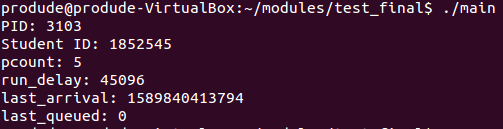
\includegraphics[scale=1]{finalTest.png}
    \end{center}
    \caption{Final test program result}
    \end{figure}
\end{center}
\section{Conclusion}
All the above sections have wrapped up my process of compiling and installing a custom kernel with implemented system call.\\
I have done this on a newer version of Ubuntu (20.04), with all same configurations,... but the kernel can not compile. So it's a recommendation to stick with Ubuntu 12.04.\\
Frequently taking snap shot (back-up) of your current state of virtual machine is also crucial for error-handling and back tracking in case things go sideways.\\\\
The code for the files that implement my system call: sys\_procsched.c for the kernel source code and procsched.c for the wrapper is also included along with this report.\\\\
\emph{Thank you for reading!}
\end{document}